\documentclass{scrartcl}
\usepackage[mathletters]{ucs}
\usepackage[utf8x]{inputenc}
\usepackage{amssymb}
\usepackage{amsmath}
\usepackage[usenames]{color}
\usepackage{hyperref}
\usepackage{wasysym}
\usepackage{graphicx}
\usepackage[normalem]{ulem}
\usepackage{enumerate}

\usepackage{listings}

\lstset{ %
basicstyle=\footnotesize,       % the size of the fonts that are used for the code
showspaces=false,               % show spaces adding particular underscores
showstringspaces=false,         % underline spaces within strings
showtabs=false,                 % show tabs within strings adding particular underscores
frame=single,                   % adds a frame around the code
tabsize=2,                      % sets default tabsize to 2 spaces
breaklines=true,                % sets automatic line breaking
breakatwhitespace=false,        % sets if automatic breaks should only happen at whitespace
}


\title{Second Wheel Holder}
\date{dinsdag 08 december 2020}
\author{}

\begin{document}

\maketitle

		\section{Second Wheel Holder}

Created vrijdag 04 december 2020



The first wheel holder wasn't good because the inserts where clamped in with the knife side so it was very hard to remove them.

In a new wheel holder the clamps got changed by new clips that can easily be removed and printed again when the design changes. 

The inner tube that slides over the motor shaft is made bigger to fit over the motor axis.



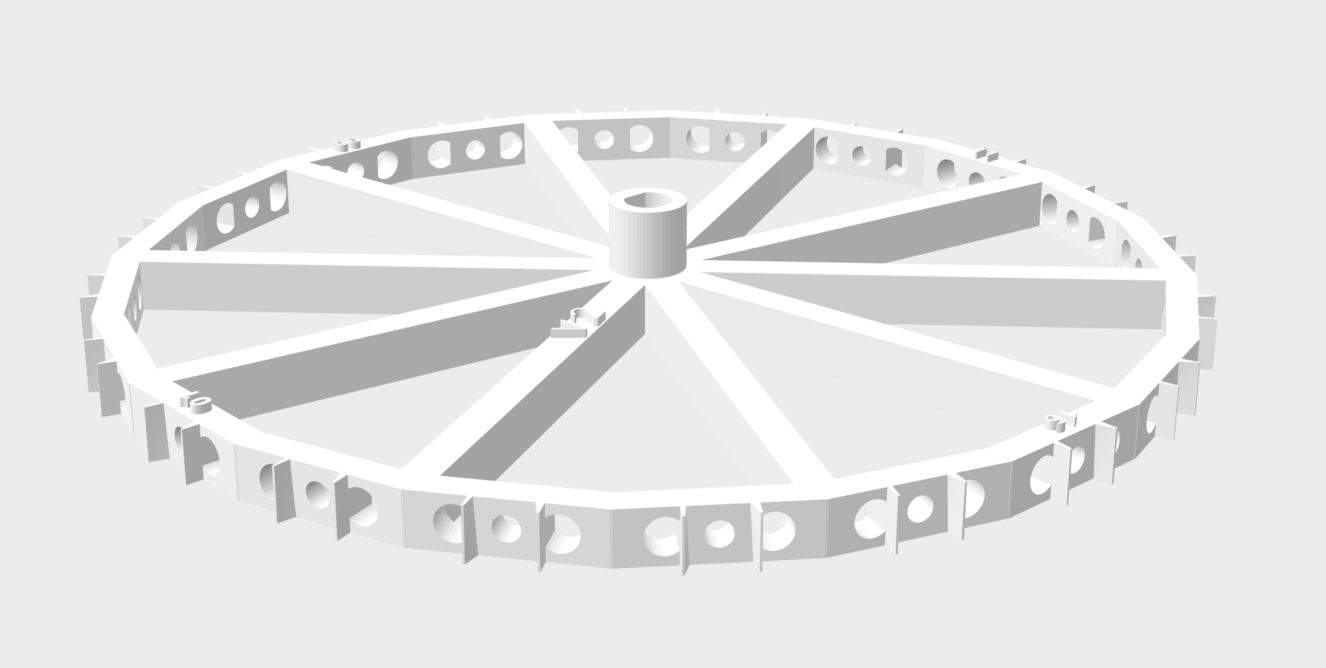
\includegraphics[width=5.208333in, keepaspectratio=true]{./Second_Wheel_Holder/radhouder_v2.png}



In the wheel there are holes in which the clips fit. The center hole is as big as the hole in the inserts. This keeps the insert from moving round the hole.

The slads between the holes are made to fit the insert perfectly so this doesn't move or shift around. 



On the pictures the slads are visible which is not ideal so they will probably have to be adjusted in a future design.



The printing of these wheels was very difficult since it was with another material as we were used to and the print wouldn't stick to the print bed. This made a few bad runs and hours of wasted printing time. At the end 8 wheels of this are printed correctly and were used to create the \href{../../../Vision/Dataset/automated_datasets/2_created_datasets/1_Birthday_dataset.tex}{Birthday dataset} and the \href{../../../Vision/Dataset/automated_datasets/2_created_datasets/2_Spaghetti_dataset.tex}{spaghetti dataset.}



The clips looked like this:

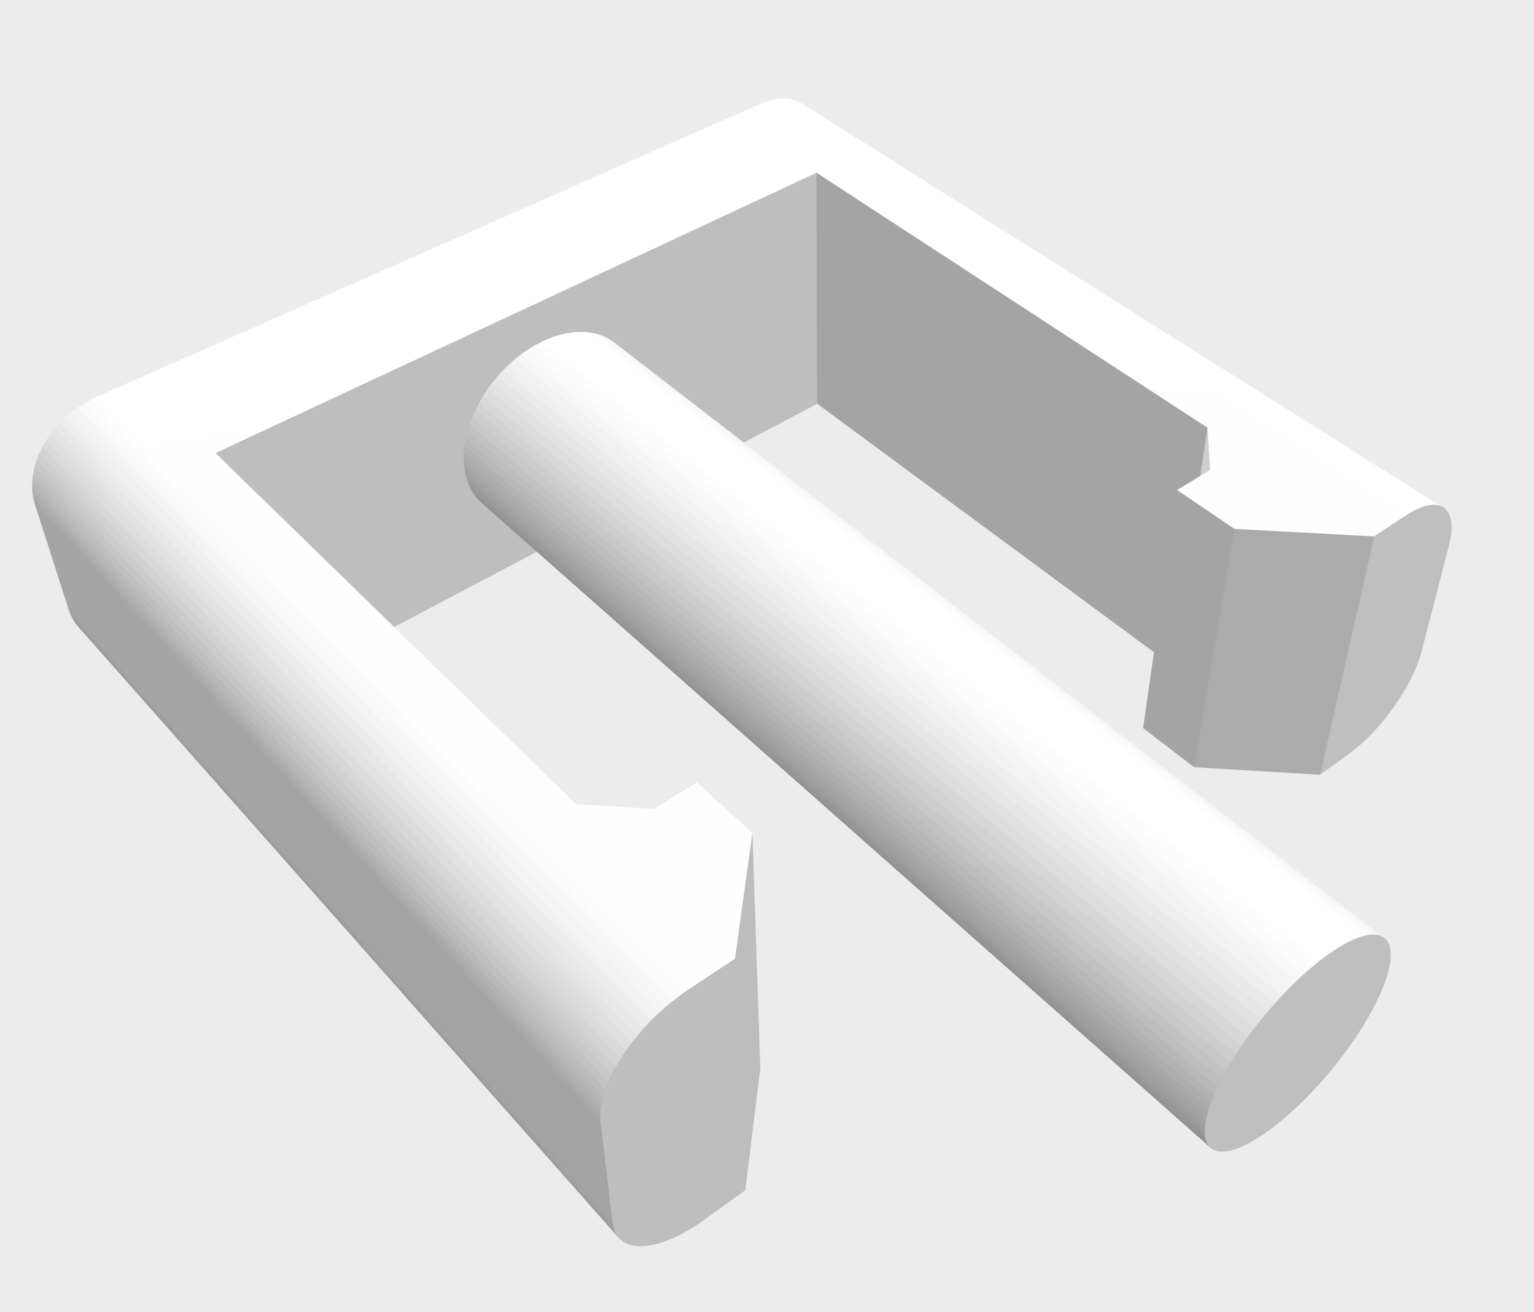
\includegraphics[width=3.125000in, keepaspectratio=true]{./Second_Wheel_Holder/clip_9.png}



\end{document}
